\documentclass[thesis]{subfiles}

\begin{document}
%*******************************************************************************
%****************************** Second Chapter *********************************
%*******************************************************************************

%Background
%• Trees, DAGs and deep neural networks (DNNs)
%• Motivation: Representing trees/DAGs as MLPs
%• Motivation: ReLUs and data routing

\chapter{Background}
\label{background}

\section{Neural Networks}
Artificial neural networks (or simply neural networks) are a broad range of statistical models characterized by consisting of a set of inter-connected nodes with non-linear \emph{activation functions} with learnable parameters, or \emph{weights}).
%, used in regression and classification problems.
 Although initially biologically inspired, Neural Networks (NN) within the field of machine learning have moved away from biologically-plausible models and towards entirely practical models guided by empirical results. Artificial neural networks are now the most popular statistical model used for learning applications in a diverse set of fields including computer vision, speech recognition, medical imagery. 

We will not cover the long and colourful history of neural networks (for this we recommend reading the introduction of~\citet{goodfellow2016deep}), but attempt to instead provide the foundations, and thereafter an overview of contemporary models and methods directly relevant to this work. For a comprehensive overview of the basics of neural networks we refer the reader to the excellent reference of~\citet{Bishop1995}, and for a more recent  in-depth overview of the field of \emph{deep learning}, we refer the reader to~\citet{goodfellow2016deep}. 

\subsection{The Neuron}

\begin{figure}[tbp]
\centering
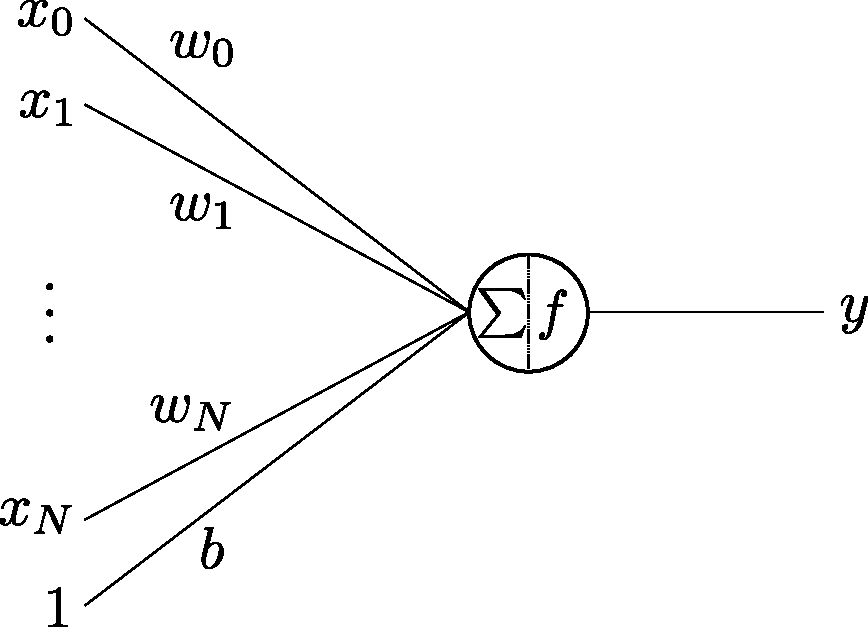
\includegraphics[width=0.5\textwidth]{neuron}
\caption[An illustration of a typical artificial neural network neuron]{An illustration of a typical artificial neural network \emph{neuron}, with output $y$, a set of inputs, $\{x_0, \ldots, x_N\}$, input weights $\{w_0, \ldots, w_N\}$, bias $b$ and activation function $f$. Here the bias $b$ is considered the weight of a fixed unit input.}
\label{fig:neuron}
\end{figure}
A neuron is a function of the weighted aggregation of its many inputs ${x_0,\ldots,x_N}$,

\begin{equation}
	y = f\left(\sum_{i}^{N} w_i x_i + b\right),
\end{equation}

where $w_i$ is the weight of the input $x_i$, and $f$ is an \emph{activation function}, and $b$ is the \emph{bias}. This is usually expressed more simply in matrix notation, where each neuron consists of an input vector $\mathbf{x}=(x_0,\ldots,x_N)$, weights $\mathbf{w}$ and a bias $b$, the output of which is, %The bias term can also be considered as the weight of an input with a fixed value of $1$, as illustrated in Fig.\,\ref{fig:neuron}.

\begin{equation}
    y = f\left(\mathbf{w}^T\mathbf{x} + b \right).
\end{equation}

If we assume the function $f$ to be a variant of the Heaviside step function,
\begin{equation}
    f(x) = 
\begin{cases}
1 & \text{if } x \geq 0\\
0 \textrm{ (or $-1$)} & \text{if } x < 0,
\end{cases}
\end{equation}

\begin{figure}[tbp]
\centering
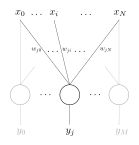
\includegraphics[width=0.5\textwidth]{singlelayer}
\caption[A single layer neural network]{An illustration of a simple single layer neural network, such as a perceptron network.}
\label{fig:singlelayer}
\end{figure}
then the neuron is also called a \emph{perceptron}, a simple binary classifier, and one of the earliest connectionist learning methods, invented by~\citet{rosenblatt1958perceptron} in 1957. A perceptron network is a single layer neural network (\ie a linear classifier), such as that illustrated in Fig.~\ref{fig:singlelayer}, and should not to be confused with a multi-layer perceptron (MLP) -- an unfortunate, but common, misnomer of any multi-layer neural network.
\begin{figure}[tbp]
\centering
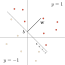
\includegraphics[width=0.5\textwidth]{perceptronline}
\caption[The interpretation of a perceptron as a hyperplane]{The interpretation of a perceptron as a oriented hyperplane, \ie a line, in $\mathbb{R}^2$.}
\label{fig:hyperplane}
\end{figure}
The perceptron also has a geometric interpretation, as shown in Fig.~\ref{fig:hyperplane}~\citet{Bishop1995}. In 2D, for example, this is equivalent to the equation of the line. Assuming our perceptron only has a single input, \ie $N=1$, if we define $a\equiv w_0$, $x \equiv x_0$, $c \equiv b$, and $f(x) = x,$

\begin{equation}
y = a x + c.
\end{equation}

In general a perceptron defines a \emph{hyperplane}, a separating manifold of dimension $d - 1$ for an input space of dimension $d$, a line in two dimensions, or plane in 3 dimensions. Neural networks are a discriminative classifier, and each neuron can be visualized as a hyperplane functioning as a single decision boundary.

\subsection{The Limitations of Single-Layer Networks}
\begin{figure}[tbp]
\centering
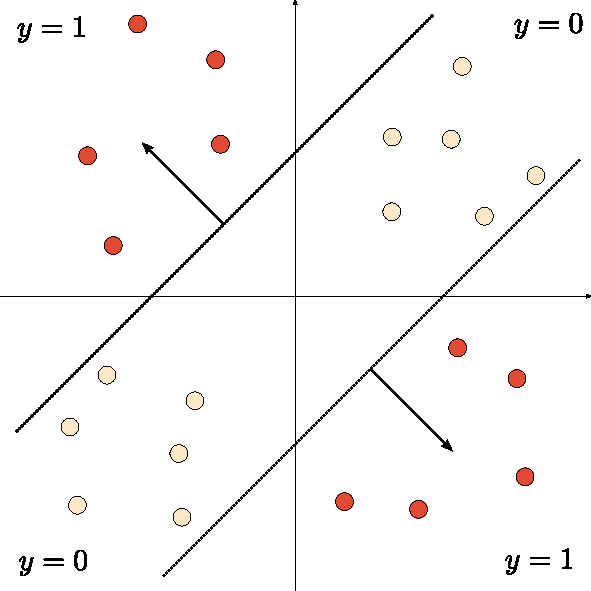
\includegraphics[width=0.5\textwidth]{perceptronxor}
\caption[An illustration of the inability of a single line to correctly classify the XOR function]{An illustration of the inability of a single line (\ie a perceptron) to correctly classify the XOR function. Instead, the composition of two lines is required to correctly separate these samples, \ie multiple layers.}
\label{fig:perceptronxor}
\end{figure}
A single layer neural network, such as the perceptron, is only a linear classifier, and as such is ineffective at learning a large variety of tasks. Most notably, in the 1969 book \emph{Perceptrons}~\citep{minsky1988perceptrons}, the authors Marvin Minsky and Seymour Papert showed that single-layer perceptrons could not learn to model functions as simple as the XOR function, amongst other non-linearly separable classification problems. As shown in Fig.~\ref{fig:perceptronxor}, no single line can separate even a sparse sampling of the XOR function -- \ie \emph{it is not linearly separable}. Instead, only a composition of lines is able to correctly separate and classify this function, and other non-linearly separable problems.

At the time, it was not obvious how to train networks with more than one layer of neurons, since the methods of learning neuron weights, the \emph{perceptron learning rule}~\citep{rosenblatt1961principles} for perceptrons or the \emph{delta rule}~\citep{widrow1960adaptive} for general neurons, only applied to single-layered networks. %This became known as the credit-assignment problem.

\subsection{Training Single Layer Networks: The Delta Rule}
\label{deltarule}
\begin{figure}[tbp]
\centering
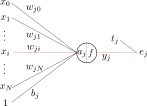
\includegraphics[width=0.5\textwidth]{neurononelayer}
\caption[Detailed illustration of a single layer neural network]{Detailed illustration of a single layer neural network trainable with the delta rule.. The input layer consists of a set of inputs, $\{x_{0}, \ldots, x_{N}\}$. The layer has weights $\{w_{j0}, \ldots, w_{jN}\}$, bias $b_j$, net neuron activity $a_j = \sum_i w_{ji}$ and activation function $f$, output $y_j$, has weights $\{w_{k0}, \ldots, w_{jN}\}$ and bias $b_j$. The error for output $y_j$, $e_j$, is calculated using the target label $t_j$.}
\label{fig:neurononelayer}
\end{figure}

The delta rule for single-layered neural networks is a gradient descent method, using the derivative of the network's weights with respect to the output error to adjust the weights to better classify training examples. As shown in the figure, we can consider the bias to be an extra weight with a unit input, and thus we can omit the explicit bias from the derivation. Assume that for a training sample $\mathbf{x}^n = (x^n_0, \ldots, x^n_i, \ldots, x^n_N)$, the $i$th neuron in our single-layer neural network has output $y^n_j$, target (desired) output $t^n_j$, weights $\mathbf{w}=(w_{j0}, w_{j1}, \ldots, w_{jM})$, as shown in Fig.~\ref{fig:singlelayer}. We want to know how to change a given weight $w_{ji}$ given the output of node $j$, 
\begin{equation}
	y_j = f\left( a_j \right),
	\label{eqn:output}
\end{equation}
where the net activation $a_j$ is,
\begin{equation}
	a_j = \sum_i w_{ji} x_{i}.
	\label{eqn:weightsum}
\end{equation}
To do so, we must use the error of our prediction for each output $y_j$ and training sample $x^n$ as compared to the known label $t_j$,
\begin{equation}
    e^n_j = t^n_j - y^n_j.
    \label{eqn:error}
\end{equation}

For this derivation, we assume the error for a single sample is calculated by the squared error. In fact, the derivation holds as long as our error function is in the form of an average~\citep{Bishop1995},
\begin{equation}
    E_n = \frac{1}{2} \sum^n_j \left(e^n_j\right)^2.
    \label{eqn:errorsum}
\end{equation}

Chain rule allows us to calculate the \emph{sensitivity} of the error to each weight $w_{ji}$ in the network,
\begin{equation}
\begin{aligned}
    \frac{\partial E^n}{\partial w_{ji}} &= \frac{\partial E^n}{\partial e^n_j}\frac{\partial e^n_j}{\partial y^n_j} \frac{\partial y^n_j}{\partial a^n_j} \frac{\partial a^n_j}{\partial w_{ji}}.
\end{aligned}
\end{equation}

Differentiating Eq.~\ref{eqn:errorsum} with respect to $e^n_j$,
\begin{equation}
\begin{aligned}
    \frac{\partial E^n}{\partial e^n_j} &= e^n_j,
\end{aligned}
\end{equation}

Eq.~\ref{eqn:error} with respect to $y^n_j$,
\begin{equation}
\begin{aligned}
    \frac{\partial e^n_j}{\partial y^n_j} &= -1,
\end{aligned}
\end{equation}

Eq.~\ref{eqn:output} with respect to $a^n_j$,
\begin{equation}
\begin{aligned}
   \frac{\partial y^n_j}{\partial a^n_j}  &= f'\left( a^n_j \right),
\end{aligned}
\label{eqn:partialdyda}
\end{equation}

and finally Eq.~\ref{eqn:weightsum} with respect to $w_{ji}$,
\begin{equation}
\begin{aligned}
   \frac{\partial a^n_j}{\partial w_{ji}} &= \frac{\partial}{\partial w_{ji}} \left( \sum_i w_{ji} x_{i} \right)\\
   &= x_i,
\end{aligned}
\label{eqn:sumonetermpartial}
\end{equation}
since only one of the terms in the sum is related to the specific weight $w_{ji}$. Thus the sensitivity is,
\begin{equation}
\label{eqn:deltasensitivity}
\begin{aligned}
    \frac{\partial E^n}{\partial w_{ji}} &= - e^n_j  f'\left( a^n_j \right) x_i.
\end{aligned}
\end{equation}

Typically what is variously called the local gradient, error, or simply \emph{delta}, is then defined,
\begin{equation}
\label{eqn:delta}
\begin{aligned}
    \delta^n_j \equiv&-\frac{\partial E^n}{\partial a^n_j}\\
    =& -\frac{\partial E^n}{\partial e^n_j}\frac{\partial e^n_j}{\partial y^n_j} \frac{\partial y^n_j}{\partial a^n_j}\\
    =& e^n_j  f'\left( a^n_j \right),
\end{aligned}
\end{equation}

such that equation \ref{eqn:deltasensitivity} can be rewritten,
\begin{equation}
\begin{aligned}
    \frac{\partial E^n}{\partial w_{ji}} &= -\delta^n_j x_i.
\end{aligned}
\end{equation}


The delta rule adjusts each weight $w_{ji}$ proportional to the sensitivity, 
\begin{equation}
\begin{aligned}
    \Delta w_{ji} &= -\gamma \frac{\partial E^n}{\partial w_{ji}},
\end{aligned}
\end{equation}

where $\gamma$ is a constant called the \emph{learning rate} or \emph{step size}. Using the delta defined in \ref{eqn:delta}, this is simply written,
\begin{equation}
\begin{aligned}
    \Delta w_{ji} &= \gamma\, \delta^n_j x_i.
\end{aligned}
\end{equation}


\subsection{Backpropagation}
The credit-assignment problem was solved with the discovery of \emph{backpropagation} (also known as the \emph{generalized delta rule}), allowing learning in multi-layer neural networks. It is somewhat controversial who first ``discovered'' backpropagation, since it is essentially the application of the chain rule to neural networks, however it's generally accepted that it was first demonstrated experimentally by \citet{rumelhartbackprop}. Although it is ``just the chain rule'', to dismiss this first demonstration of backpropagation in neural networks is to understate the importance of this discovery to the field, and to dismiss the practical difficulties in first implementing the algorithm -- a fact that will be attested to by anyone who has since attempted.

Following is a derivation of backpropagation loosely based on the excellent references of \citet{haykin1994neural,Bishop1995}, although with different notation. Indeed the notation is the hardest part of the derivation, and it is important to pay attention to Fig.~\ref{fig:neurontwolayer} to understand the indexing we will use to refer to neurons of different layers, and which notably differs from that in Fig.~\ref{fig:neurononelayer} for the single layer case.

We are interested in finding the sensitivity of the error $E$ to a given weight in the network $w_{ij}$. There are two classes of weights for which we must derive different rules, 
\begin{enumerate*}[label=(\textbf{\roman*})]
  \item \label{enum:outputneuron} those belonging to \emph{output layer neurons}, \ie neurons lying directly before the output, such as $w_{kj}$ in Fig.~\ref{fig:neurontwolayer}, and
  \item \label{enum:hiddenneuron} weights belonging to hidden layer neurons, such as $w_{ji}$ in Fig.~\ref{fig:neurontwolayer}.
\end{enumerate*}

\paragraph{\ref{enum:outputneuron}~Output Layer.}
The output weights are relatively easy to find, since they correspond to the same types of weights found in single layer networks, and have direct access to the error signal, \ie $e^n_j$. Indeed the derivation in \S\ref{deltarule} also describes the sensitivity of the weights in the output layer of a multi-layer neural network. With some change of notation (now indexing by $k$ rather than $j$ to match Fig.~\ref{fig:neurontwolayer}), we can use the sensitivity found in Eqn.~\ref{eqn:deltasensitivity},

\begin{equation}
\begin{aligned}
    \frac{\partial E^n}{\partial w_{kj}} &= \frac{\partial E^n}{\partial a^n_k} \frac{\partial a^n_k}{\partial w_{kj}}\\
%    \frac{\partial E^n}{\partial w_{kj}} &= \frac{\partial E^n}{\partial e^n_k}\frac{\partial e^n_k}{\partial y^n_k} \frac{\partial y^n_k}{\partial a^n_k}\\
%    &= - e^n_k  f'\left( a^n_k \right) x^n_{kj}\\
    &= -\delta^n_k x^n_{kj}\\
    &= -\delta^n_k y^n_j.
\end{aligned}
\label{eqn:outputlayer}
\end{equation}

\paragraph{\ref{enum:hiddenneuron} Hidden Layer.}
\begin{figure}[tbp]
\centering
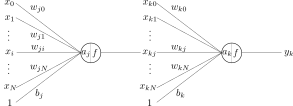
\includegraphics[width=0.8\textwidth]{neurontwolayer}
\caption[An illustration of a neural network with a single hidden layer]{An illustration of a neural network with a single hidden layer. The input layer consists of a set of inputs, $\{x_{0}, \ldots, x_{N}\}$. The hidden layer has weights $\{w_{i0}, \ldots, w_{iN}\}$, bias $b_i$, net neuron activity $a_j = \sum_i w_{ji}$ and activation function $f$. The output layer with output $y_k$, has weights $\{w_{k0}, \ldots, w_{jN}\}$ and bias $b_j$. The error for output $y_k$, $e_k$, is calculated using the target label $t_k$. Note that $x^n_{kj} \equiv y^n	_j$.}
\label{fig:neurontwolayer}
\end{figure}
We will first derive the partial derivative ${\partial E^n}/{\partial w_{ji}}$, for a single hidden layer network, such as that illustrated in Fig.~\ref{fig:neurontwolayer}. Unlike in the first case, the weights belonging to hidden neurons have no direct access to the error signal, instead we must calculate the error signal from all the neurons that indirectly connect the neuron to the error (\ie every output neuron $y_k$).

Following from chain rule we can write the partial derivative of a hidden weight $w_{ji}$ with respect to the error $E$,
\begin{equation}
\begin{aligned}
    \frac{\partial E^n}{\partial w_{ji}} &= \underbrace{\left( \sum_k \frac{\partial E^n}{\partial e^n_{k}}
     \frac{\partial e^n_{k}}{\partial y^n_{k}} \frac{\partial y^n_{k}}{\partial a^n_k} \frac{\partial a^n_k}{\partial y^n_{j}}\right)}_\text{output neurons}
     \underbrace{\frac{\partial y^n_{j}}{\partial a^n_{j}} \frac{\partial a^n_{j}}{\partial w_{ji}}}_\text{hidden neuron},
     \label{eqn:twolayer1}
\end{aligned}
\end{equation}

where the sum arises from the fact that, unlike in Eq.~\ref{eqn:sumonetermpartial} where the weight $w_{kj}$ affects only a single output, the hidden weight $w_{ji}$ affects all neurons in the subsequent layer (see Fig.~\ref{fig:neurontwolayer}).

We already know how to calculate the partials for the output layer from the derivation of the delta rule for single-layer networks, and we can substitute these from Eq.~\ref{eqn:outputlayer} for the output neuron and error partial derivatives,

\begin{equation}
\begin{aligned}
    \frac{\partial E^n}{\partial w_{ji}} &= -\left( \sum_k \delta^n_k y^n_j \frac{\partial a^n_k}{\partial y^n_{j}}\right)
     \frac{\partial y^n_{j}}{\partial a^n_{j}} \frac{\partial a^n_{j}}{\partial w_{ji}}.
     \label{eqn:twolayer2}
\end{aligned}
\end{equation}

Recall from Eq.~\ref{eqn:weightsum}, the net activation $a$ is a sum of all previous layer weights. Thus,
\begin{equation}
\begin{aligned}
    \frac{\partial a^n_k}{\partial y^n_{j}} &= \frac{\partial}{\partial y^n_{j}}\left(\sum_j w_{kj} y^n_{j} \right) &= w_{kj},
\end{aligned}
\end{equation}

and substituting from Eq.~\ref{eqn:partialdyda} and Eq.~\ref{eqn:sumonetermpartial} into Eq.~\ref{eqn:twolayer2},
\begin{equation}
\begin{aligned}
    \frac{\partial E^n}{\partial w_{ji}} &= -\left( \sum_k \delta^n_k y^n_j w_{kj}\right)
     f'\left( a^n_j \right) x_i.
     \label{eqn:twolayer3}
\end{aligned}
\end{equation}

This bears some resemblance to the derived expression for a single layer, and just as in Eq.~\ref{eqn:delta}, we can use our definition of the delta to simplify it. For hidden layers this evaluates as,
\begin{equation}
\label{eqn:deltahidden}
\begin{aligned}
    \delta^n_j \equiv& \frac{\partial E^n}{\partial a^n_k}\\
    =& -\left( \sum_k \frac{\partial E^n}{\partial e^n_{k}} \frac{\partial e^n_{k}}{\partial y^n_{k}} \right) \frac{\partial y^n_{k}}{\partial a^n_k}\\
    =& -\left(\sum_k \delta^n_k y^n_j w_{kj} \right) f'\left( a^n_j \right).
\end{aligned}
\end{equation}

This leaves us with the more convenient (as we will see in \S\ref{arbitraryhidden}) expression,
\begin{equation}
\begin{aligned}
    \frac{\partial E^n}{\partial w_{ji}} &=  \delta^n_j x_i.
     \label{eqn:twolayer4}
\end{aligned}
\end{equation}

\subsubsection{Arbitrary Number of Hidden Layers}
\label{arbitraryhidden}
The derivation above was based on the specific case of a single hidden layer network, but it is trivial to extend this result to multiple hidden layers. There is a recursion in the calculation of the partial derivatives in Eq.~\ref{eqn:deltahidden} which holds for a network with any number of hidden layers, and which we will now make explicit. 

The delta is defined,
\begin{equation}
\delta^n_i = \begin{cases}
         e^n_j \, f'\left( a^n_j \right)& \textrm{when neuron $j$ is output}\\
        - \left( \sum_j \delta^n_j y^n_i w_{ji} \right) f'\left( a^n_j \right)& \textrm{when neuron $j$ is hidden},
        \end{cases}
\label{eqn:fulldeltadefinition}
\end{equation}
for any adjacent neural network layers $i, j$, including the output layer where the outputs are considered to have an index $j$. The sensitivity is then, 
\begin{equation}
\begin{aligned}
    \frac{\partial E^n}{\partial w_{ji}} &=  \delta^n_j y_i.
     \label{eqn:sensitivity}
\end{aligned}
\end{equation}

\mynote{Finish backprop derivation}


\subsubsection{Learning with Backpropagation}
Learning with backpropogation is much like the delta rule; sensitivities are used to correct weights proportional to a constant \emph{learning rate} or \emph{step size} parameter $\lambda$. Formally, the weight change rule is given by,
\begin{equation}
\begin{aligned}
    \Delta w^n_{ij} &= \lambda\, \frac{\partial E^n}{\partial w_{ji}}\\
    &= \lambda \, \delta^n_j y_i,
     \label{eqn:backproplearningrule}
\end{aligned}
\end{equation}
where $\delta^n_j$ is as defined in Eq.~\ref{eqn:fulldeltadefinition}, and $y_i$ is the output of neuron $i$.

\subsection{Online, Batch and Stochastic Gradient Descent}
Although the backpropagation weight change rule above tells us how to change the weight given a single training sample $n$, in practice this method, called \emph{online training}, is rarely used. The reason is simply that the gradients from a single sample are too biased, or noisy, and they are not representative of the dataset in general.

At the opposite end of the spectrum there is \emph{batch training} where the gradient is based on all data samples in the training set,
\mynote{TODO define this formally}.

Although this gives a very good gradient, it is very expensive to compute, since it requires us to perform the forward pass of the network over all training samples. It has also been observed in practice that adding noise to the gradient at training time helps generalization, perhaps by preventing overfitting.

InsteadAnother form of training is called 
\mynote{TODO}

\subsection{Activation Functions}
As we have seen with the perceptron, the activation function for a single-layer network can provide a means of pushing the outputs of each neuron towards a binary classification. However the activation function has a much more important function in multi-layer neural networks. Without a non-linear activation function, even a large multi-layer neural network would only have the representational power of a linear classifier -- the composition of linear functions is a linear function. For this reason, the \emph{activation function} $f$ is a non-linear function applied to the output of a neuron to allow multi-layer networks to learn complex non-linear functions,

\begin{equation}
y = f\left(\mathbf{w}^T\mathbf{x} + b\right).
\end{equation}

In the field of neural networks, activation functions have classically chosen to be a \emph{sigmoid} function, \ie a function mapping negative inputs to negative outputs and positive inputs to positive outputs with a smooth transition around $a = 0$. This is a nice property to have, since the function is still pushing the outputs of the network towards a binary classification, the function is non-linear (so composition of functions are non-trivial), and the function has well-defined and gradients. Examples of sigmoid functions commonly used include the logistic function, 

\begin{equation}
	f(x) = \frac{1}{1+e^{-x}},
\end{equation}

and they hyperbolic tangent,
\begin{equation}
	f(x) = \tanh(x).
\end{equation}

An issue with sigmoidal activations functions however, is that the gradients are very small in a large part of the domain of the function. For this reason, and improved empirical results, modern neural networks tend to use the \emph{ReLU} activation function, as described in \S\ref{section:relu}.


\subsection{Hidden Layers}
\mynote{Fill this in more}Neural networks with at least one (infinitely wide) \emph{hidden} layer have been proven to be a universal approximator - \ie such a neural network can theoretically represent any function~\citep{journals/mcss/Cybenko92,hornik89a}. In practice however, a network with only a single hidden layer, of even a very large width, has trouble learning to represent complex functions as compared to networks with many hidden layers layers. Networks with many hidden layers, or \emph{deep} networks, empirically achieve better accuracy than networks with few hidden layers, or \emph{shallow} networks.

\subsection{Convolutional Neural Networks}
The earliest work on what are now termed \emph{Convolutional Neural Networks} (CNNs) was by~\citet{Fuk80}, on the \emph{Neocognitron}~\citep{fukushima2013artificial}. The neocognitron was a biologically motivated architecture, motivated by what are typically called simple and complex cells in the primary visual cortex (V1). To model simple cells; cells whose response correlated with simple oriented edges in a translation invariant manner, the neocognitron used shared weights which were connected to local image patches of the input image (and were not simply described as convolution of a filter). Complex cells were modelled by a ``blurring'' operation, what we now term more generally as \emph{pooling}. The neocognitron network consisted of alternating layers of simple and complex cells, \ie alternating convolution and pooling layers, much as seen in state of the art convolutional networks.

Despite the pioneering novelty of the work on neocognitrons, it was only following the simplification and improvement of~\citet{Lecun1998} in both the description of the network and its operation that it gained wider acknowledgement as a breakthrough for image recognition. In their work the local shared weights of the neocognitron are put in the context of convolution, and the averaging operation replaces with max-pooling. The application to handwritten digit recognition gave state of the art results, and would result in the \emph{LeNet5} network, still used today in commercial applications.

The application of the LeNet-style CNN architecture to more complex problems, however, proved infeasible. These problems required a deeper hierarchy of representation, which implied a large number of layers. Networks with a large number of layers proved to be un-trainable due to numerous issues with the model itself, notably vanishing gradients~\citep{hochreiter1991untersuchungen}, and the lack of large datasets and computational power at the time. Convolutional neural networks fell out of favour, and were passed over in favour of the more successful paradigm of using hand-crafted local features for many tasks, and in particular the problem of object instance recognition was well addressed by such solutions. Meanwhile object class recognition remained a difficult problem, for which the best solutions were deformable parts models, also based on local features.

\subsubsection{Convolution Layers}
\begin{figure}[tb]
	\centering
	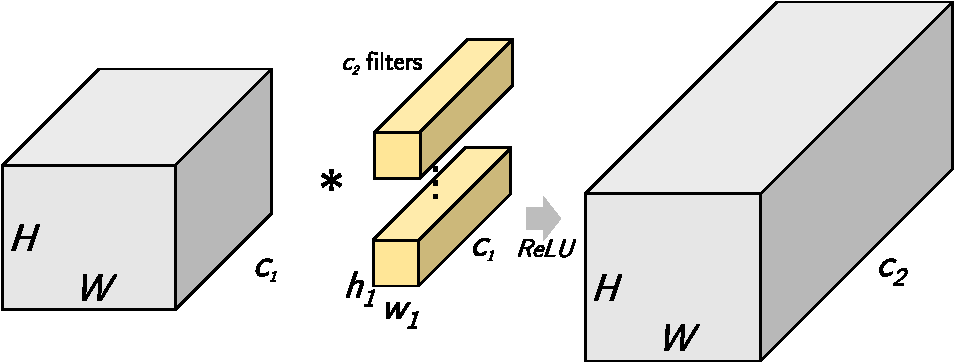
\includegraphics[width=0.66\columnwidth, page=1]{groupfig}
	\caption[Illustration of convolutional layer]{\textbf{Convolution with $d$ filters of shape $h\times w\times c$.} Convolutional filters (yellow) have the same channel dimension $c$ as the input feature maps (gray) on which they operate. Each filter is convolved across the entire set of input featuremaps to produce a single output feature map. In this illustration we assume padding appropriate to preserve the spatial dimensions.}
	\label{fig:convlayer}
\end{figure}

Figure \ref{fig:convlayer} illustrates a typical convolutional layer. If we denote the $d^{\text{th}}$ feature map for the given layer as $h^d$, where the associated filter has weights $W^d$, bias $b_d$, and activation function $f$, then the single \emph{pixel} of the feature map $h^d$ at spatial location $i, j$ is given by,

\begin{equation}
	h^d_{i,j} = f\left( \left(W^d \convolution x \right)_{i,j} + b_d \right),
\end{equation}

where $\convolution$ is the convolution operator. The discrete convolution operator $(f \convolution g)$ is defined~\citep{damelin2011} for two 1D sequences $f, g$ as,
\begin{equation}
	(f \convolution g)[n] = \sum_{i=-\infty}^\infty f[i]\, g[n - i].
\end{equation}

This can be extended to 2D sequences,
\begin{equation}
(f \convolution g)[m,\,n] = \sum_{i=-\infty}^\infty \sum_{j=-\infty}^\infty f[i,\,j]\, g[m - i][n - j].
\end{equation}

\subsubsection{Pooling Layers}
Another key aspect of convolutional architectures is pooling, a form of non-linear spatial sub-sampling of the feature maps of a given layer. Pooling layers were designed to add translation invariance to CNNs by making the network less sensitive to small local changes in the spatial location of input pixels/convolutional responses, and also to reduce feature map spatial sizes with network depth. Reducing the feature map spatial size serves both to save computation, and to increase the size of the receptive field of successive convolutional layers. This allows successive convolutional layers to operate on progressively larger scales.

Pooling layers divide the image into non-overlapping pooling regions, in which the spatial extents of the input image/feature map are aggregated into a single scalar. LeNet used the average to aggregate the pooling regions, \ie average pooling~\citep{Lecun1998}. More modern networks have typically used max to aggregate pooling regions, \ie max-pooling which empirically has been found to work better. Some even more recent networks do not use pooling at all, but simply use a strided convolution to reduce the feature map sizes~\citep{He2015}.

\section{Contemporary Methods of Training Deep Neural Networks}
\label{section:contemporary}
\subsection{Rectified Linear Activation Function}
\label{section:relu}
An integral part of any useful neuron in a neural network is a non-linear activation function. With a linear activation function, even the deepest network would only be able to represent a linear function. Historically, neural networks have used sigmoidal activation functions. These functions include the hyperbolic tangent ($f(x) = \tanh(x)$), as plotted in Fig.~\ref{fig:tanh} and logistic function ($f(x) = \frac{1}{1+e^{-x}}$). Both of these functions have the nice properties that their range is normalized in ($[-1,1]$ in the case of the hyperbolic tangent), and they are smooth functions with easy to calculate derivatives.

\begin{figure}[tbp]
	\centering
	\begin{subfigure}[t]{0.48\textwidth}
		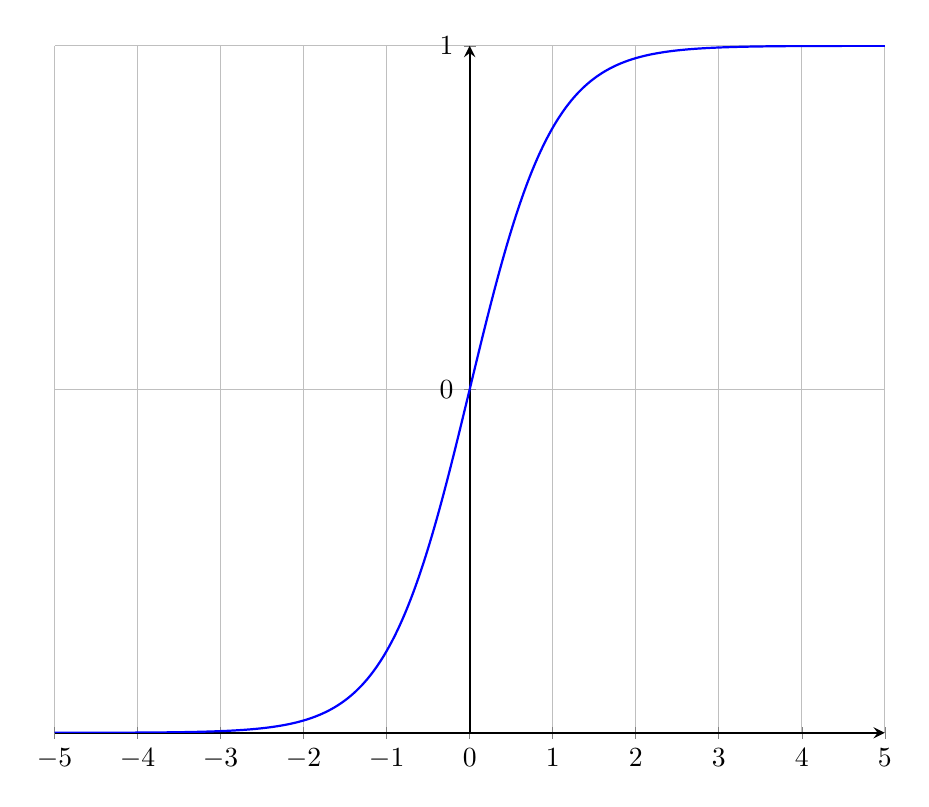
\begin{tikzpicture}
		\begin{axis}%
		[
		thick,
		width=\textwidth,
		height=0.85\textwidth,
		grid=major,
		xmin=-5,
		xmax=5,
		axis x line=bottom,
		ytick={-1,0,1},
		ymax=1,
		ymin=-1,
		axis y line=middle,
		]
		\addplot%
		[
		blue,%
		mark=none,
		samples=500,
		domain=-5:5,
		]
		(x,{tanh(x)});
		\end{axis}
		\end{tikzpicture}
		\caption{Hyperbolic Tangent $y = \tanh(x)$}
		\label{fig:tanh}
	\end{subfigure}
	~
	\begin{subfigure}[t]{0.48\textwidth}
		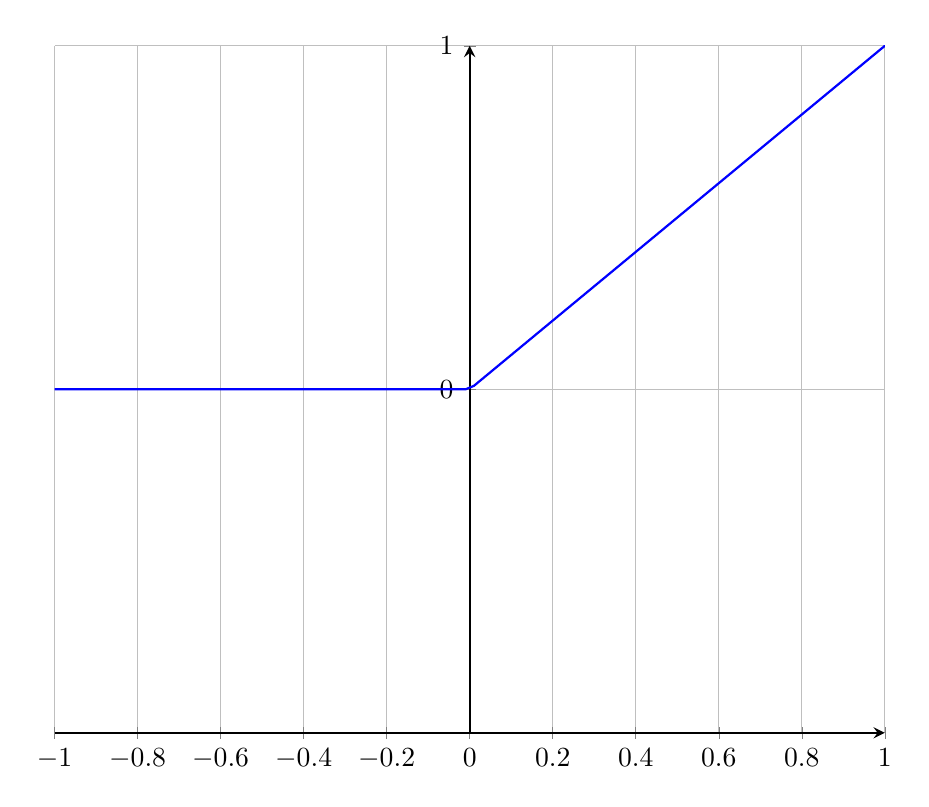
\begin{tikzpicture}
		\begin{axis}%
		[
		thick,
		width=\textwidth,
		height=0.85\textwidth,
		grid=major,
		xmin=-1,
		xmax=1,
		axis x line=bottom,
		ytick={-1,0,1},
		ymax=1,
		ymin=-1,
		axis y line=middle,
		]
		\addplot%
		[
		blue,%
		mark=none,
		samples=500,
		domain=-5:5,
		]
		(x,{max(x,0)});
		\end{axis}
		\end{tikzpicture}
		\caption{ReLU activation function $y = \max(0,x)$}
		\label{fig:relu}
	\end{subfigure}\\
	\begin{subfigure}[t]{0.48\textwidth}
		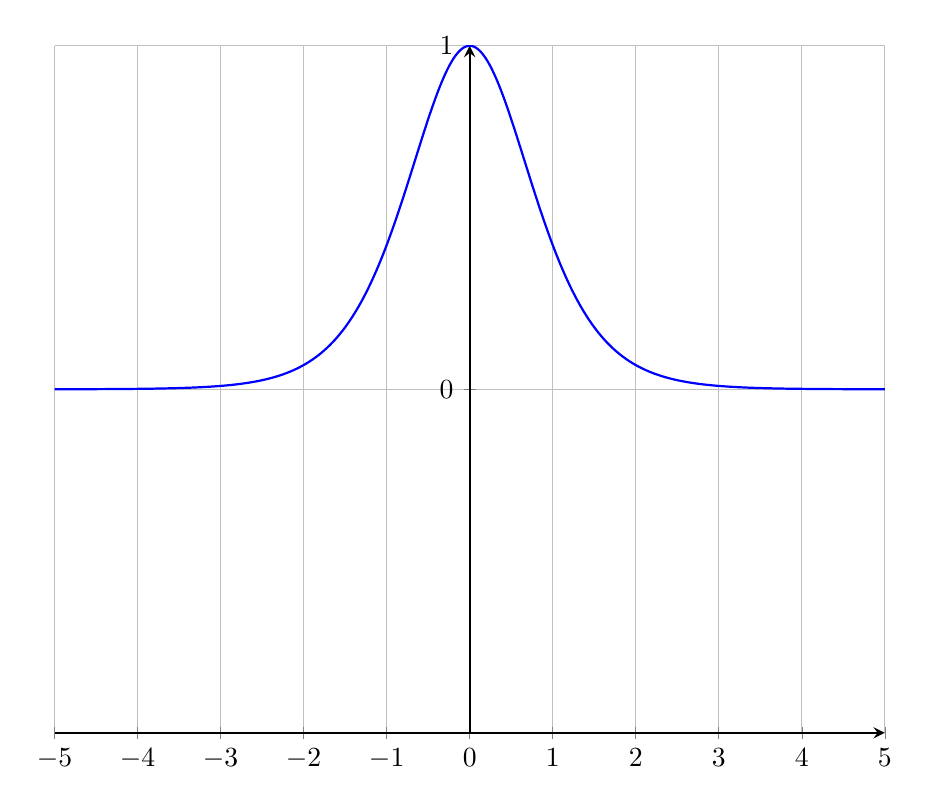
\begin{tikzpicture}
		\begin{axis}%
		[
		thick,
		width=\textwidth,
		height=0.85\textwidth,
		grid=major,
		xmin=-5,
		xmax=5,
		axis x line=bottom,
		ytick={-1,0,1},
		ymax=1,
		ymin=-1,
		axis y line=middle,
		]
		\addplot%
		[
		blue,%
		mark=none,
		samples=500,
		domain=-5:5,
		]
		(x,{1-tanh(x)*tanh(x)});
		\end{axis}
		\end{tikzpicture}
		\caption{Derivative $\frac{d\tanh(x)}{dx}$}
		\label{fig:tanhgradients}
	\end{subfigure}
	~
	\begin{subfigure}[t]{0.48\textwidth}
		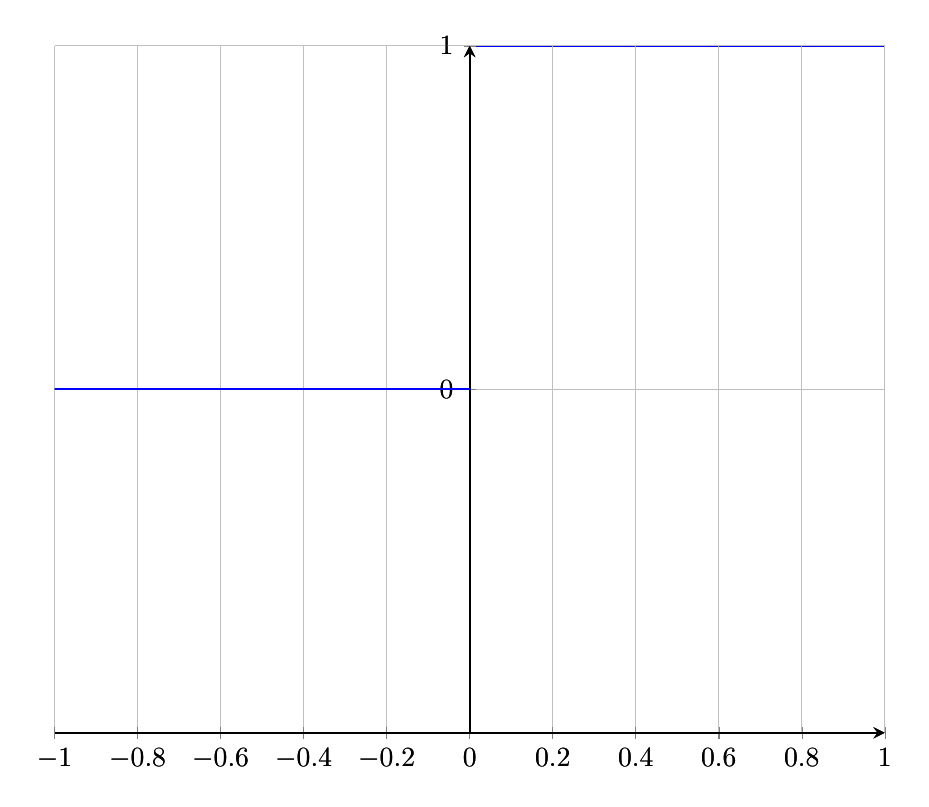
\begin{tikzpicture}[
		declare function={
		  	func(\x) = (\x<=0) * (0) + and(\x>0) * (1);
		 }
		]
		\begin{axis}%
		[
		thick,
		width=\textwidth,
		height=0.85\textwidth,
		grid=major,
		xmin=-1,
		xmax=1,
		axis x line=bottom,
		ytick={-1,0,1},
		ymax=1,
		ymin=-1,
		axis y line=middle,
		]
		\addplot%
		[
		blue,%
		mark=none,
		samples=500,
		domain=0:5,
		]
		(x, {1});
		\end{axis}
		\begin{axis}%
		[
		thick,
		width=\textwidth,
		height=0.85\textwidth,
		grid=major,
		xmin=-1,
		xmax=1,
		axis x line=bottom,
		ytick={-1,0,1},
		ymax=1,
		ymin=-1,
		axis y line=middle,
		]
		\addplot%
		[
		blue,%
		mark=none,
		samples=500,
		domain=-5:0,
		]
		(x, {0});
		\end{axis}
		\end{tikzpicture}
		\caption{Derivative $\frac{d \max(0,x)}{dx}$}
		\label{fig:relugradient}
	\end{subfigure}
	\caption[Activation Functions]{Activation functions for Neural Networks}
	\label{fig:afunctions}
\end{figure}

A major issue with sigmoidal activation functions however, is that gradients outside of a relatively narrow region of the function domain (close to $x=0$) are very small. When training with back propagation, this means that most gradients are of very small magnitude, and training can take a very long time, or even stall altogether -- a situation that is often called the \emph{vanishing gradient} problem, first identified by \citet{hochreiter1991untersuchungen}. This term has also been conflated with numerical precision issues caused by incorrect initialization, as identified by \citet{glorot2010understanding}.

Rectified linear units (ReLU) were proposed as a solution, first for restricted Boltzmann machines~\citep{conf/icml/NairH10}, and later for neural networks~\citep{glorot2010understanding}, where empirically they were shown to allow easier training with backpropagation. These neurons have a piecewise activation function, $f(x) = \max(0,x)$ (Fig.~\ref{fig:relu}). ReLUs do not exhibit the `saturation' of sigmoidal functions, always giving a gradient of either 0 or 1. In practice this can greatly speed up training with back propagation, or even allow training networks that are not trainable in practice with sigmoidal activation functions, such as the deep network of \citet{Krizhevsky2012}.

\subsection{Methods of Network Initialization}\label{ssec:init}
Until relatively recently, pre-training was considered necessary for the feasibility of training deep neural networks~\citep{hinton2006reducing}. The vanishing gradient problem was first addressed through better methods of random initialization which considered the geometric effect of propagating gradients through very deep networks. Without careful initialization, gradients can either surpass numerical representation (exploding gradients) or be reduced to close to zero (vanishing gradients). This effect is further exacerbated by the use of the softmax function at the end of the network, containing the exponential function.

For example, consider a deep network consisting of $L$ identical layers as shown in Fig.~\ref{fig:manylayers}, and assume that our initialization results in the first pass through the network scaling the signal (i.e~gradients) by a factor of $\beta$ for each layer.

After propagating through $L$ layers, this becomes a scaling of $\beta^L$, greatly magnifying the effect of the discrepancy. For example, the output of a trivial deep network  where each layer $l$ only maps the identity function, $f_{l}(x) = x$, with $L$ layers, and each layer initialized such that the output response is scaled by $\beta$:

\begin{figure}[tbp]
	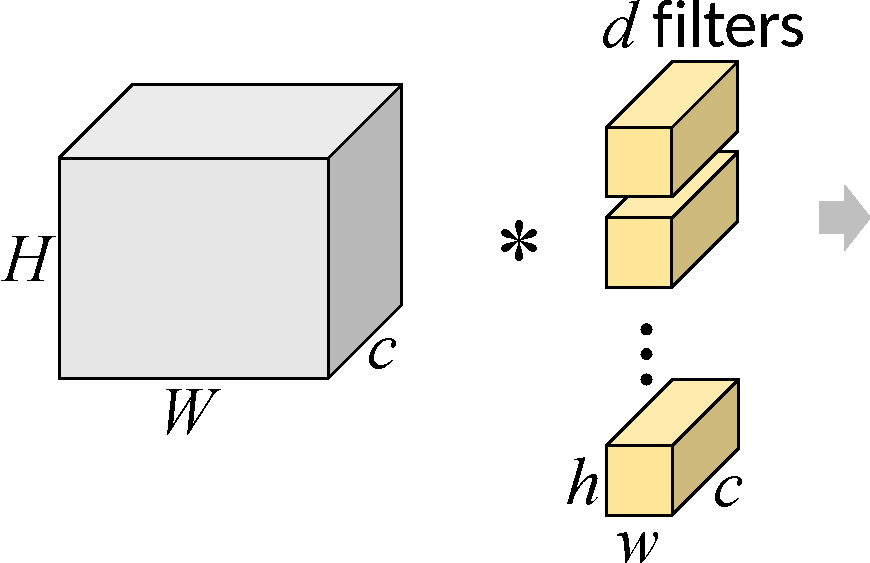
\includegraphics[width=0.23\textwidth, page=1, viewport = 0 0 440 600, clip=true]{layer}
	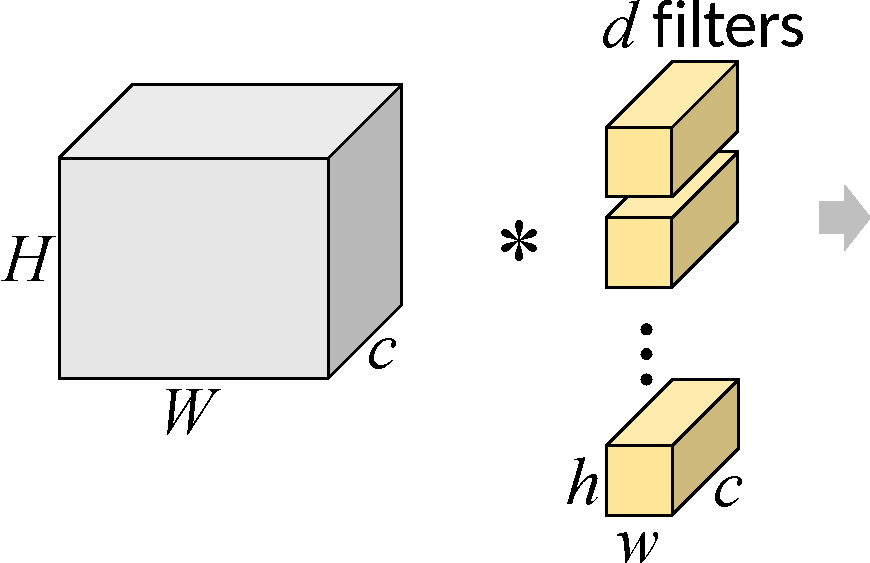
\includegraphics[width=0.23\textwidth, page=1, viewport = 0 0 440 600, clip=true]{layer}
	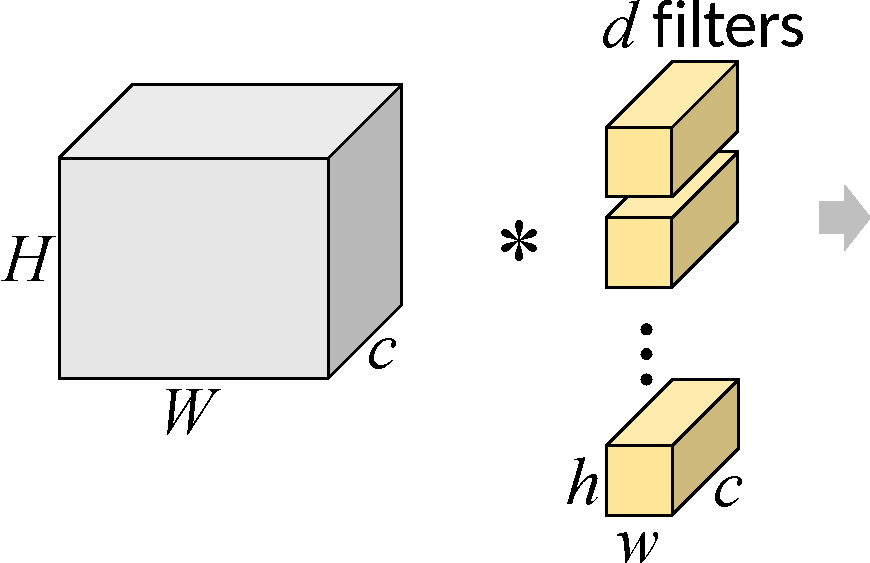
\includegraphics[width=0.23\textwidth, page=1, viewport = 0 0 440 600, clip=true]{layer}
	$\cdots$
	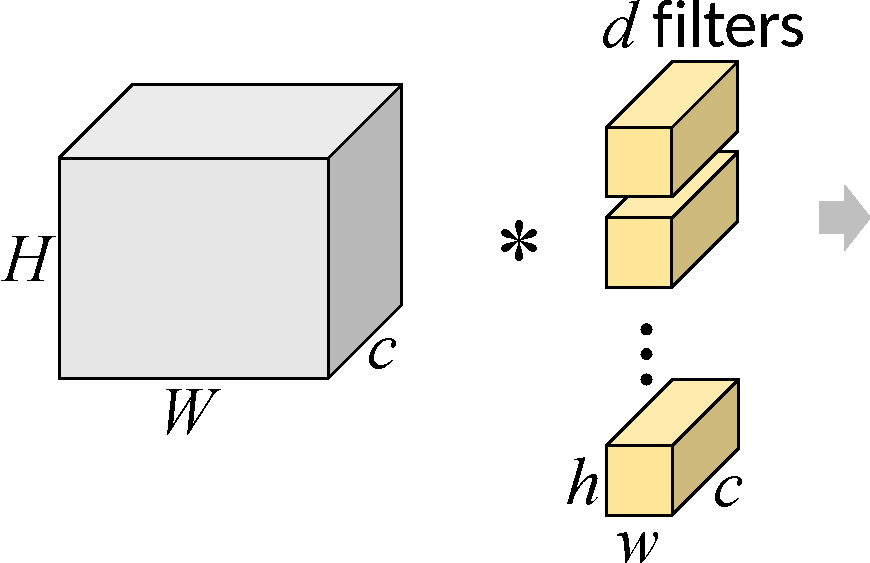
\includegraphics[width=0.23\textwidth, page=1, viewport = 0 0 400 600, clip=true]{layer}
	\caption[Vanishing Gradients]{\textbf{Vanishing Gradients.} For networks with many layers, even small deviations from a unit gradient are quickly geometrically magnified by propagation through all layers.}
	\label{fig:manylayers}
\end{figure}
\begin{equation}
\begin{aligned}
	f_L(x) & = (f_1 \circ f_2 \ldots \circ f_L) (x)\\
	& = x \, \prod^{L}_{l} \beta = x\, \beta^L
\end{aligned}
\end{equation}

\[
\lim_{L\to\infty} f_L(x) = 
\begin{cases}
\infty & \text{if } \beta > 1, \text{ training loss \emph{diverges}}\\
0 & \text{if } \beta < 1, \text{ training loss \emph{stalls}},
\end{cases}
\]

where $(f \circ g)(x)$ is the composition $f(g(x))$.

Thus we want a random initialization of layers such that $\beta\approx 1$ to minimize the 'vanishing gradient' effect. For sigmoidal activation functions, such an initialization was proposed by Glorot et al.~\citep{glorot2010understanding}. For random Gaussiaan initialization, and given the number of outgoing/incoming connections to each neuron, we can carefully choose the standard deviation $\sigma$ such that $\mathbf{E}(\beta) = 1$. 

In practice however, most networks have layers of different numbers of neurons. In this case, since there are different numbers of incoming connections and outgoing connections for each neuron, there are two possible initializations, one for the expected forward pass (response) scaling, and one for the backwards pass (gradient). As a compromise, Glorot et al.~\citep{glorot2010understanding} proposed to use the average number of outgoing and incoming connections to the neuron:

\begin{equation}
\begin{aligned}
	\sigma_{\textrm{forwards}} &= \frac{1}{\sqrt{n_{\text{out}}}},\\
	\sigma_{\textrm{backwards}} &= \frac{1}{\sqrt{n_{\text{in}}}},\\
	\sigma_{\textrm{average}} &= \frac{1}{\sqrt{(n_{\text{out}} + n_{\text{in}})/2}}.
\end{aligned}
\end{equation}

For the more typically used rectified linear unit, a variation of this initialization was proposed by He et al.~\citep{He2015b}:

\begin{equation}
\begin{aligned}
	\sigma_{\textrm{forwards}} &= \frac{2}{\sqrt{n_{\text{out}}}},\\
	\sigma_{\textrm{backwards}} &= \frac{2}{\sqrt{n_{\text{in}}}},\\
	\sigma_{\textrm{average}} &= \frac{2}{\sqrt{(n_{\text{out}} + n_{\text{in}})/2}}.
\end{aligned}
\end{equation}

\subsection{Batch Normalization}
Some network architectures are sufficiently complex, e.g.~networks with neurons with drastically different number of outgoing/incoming connections, that even careful initialization will not prevent vanishing gradients. Instead, a more direct approach of managing gradient amplitude during training was introduced by \citet{Ioffe2015}. Most state-of-the-art supervised deep networks now use both of these methods.

Batch normalization uses batch statistics to whiten the responses of layers it is applied to during training. Batch normalization calculates the the mini-batch mean and variance, and prevents vanishing gradients by normalizing responses/gradients according to the batch statistics. 

\section{Contemporary Deep Neural Networks}

\subsection{AlexNet}
Training \emph{deep} networks, that is neural networks with many (\eg 2 or more) hidden layers, had proven difficult due to the high computational complexity, and the so called ``vanishing gradient'' problem~\citep{bengio:ieeenn94}. However, recent advances have made training deep neural networks possible. \citet{Krizhevsky2012} used a combination of these advances to show that a deep convolutional network (since referred to as AlexNet) with appropriate initialization~\citep{Sutskever2013momentum}, weight decay, ReLU activation functions~\citep{conf/icml/NairH10} and drop out regularisation~\citep{Hinton2012} could beat state of the art methods on large scale object class recognition methods based on hand-crafted features by a large margin. 

AlexNet notably used training-time and test-time augmentation to achieve its state of the art accuracy. During training random $224 \times 224$ crops of a $256 \times 256$ image are used, along with random mirroring of these crops. In addition \emph{relighting augmentation} is used, where the PCA components over all RGB pixels in the image are used to perturb the ``brightness'' of the image, and give some robustness to photometric variations in the test images. At test time ``$10\times$ oversampling'' is used, that is for each $256\times 256$ test image, and its mirrored image, 4 corner and one centre crop are pushed through the network, and the prediction is simply the averaged over these 10 crops. Finally, for the best results reported (Top-5 error of 15.4\%), an \emph{ensemble} of 7 models is used, where the prediction is the average of all these models. 

AlexNet uses two filter groups throughout most of the layers of the model in order to split computation and model parameters across two GPUs, the motivation being that at the time GPUs did not have enough memory to fit such a large model. The authors observed that the filters on each GPU appeared to specialize to learn fundamentally different features regardless of initialization~\citep{Krizhevsky2012}. This interesting observation has mostly been ignored in subsequent networks where GPU memory has increased enough that such a split of the network is not required, but the original observation is a fundamental motivation of our work.

\subsection{Network in Network}
\citet{Lin2013NiN} introduced \emph{Network in Network} (NiN), in which the main contribution was the use of so called `micro networks', consisting of increased non-linearity between convolutions using 1$\times$1 convolutions. The authors claimed extra the non-linearities introduced allow the network to capture more complex functions. These 1$\times $1 convolutions have since been referred to as \emph{low dimensional embeddings}, \ie a reduction in the number of filters by a mapping of a high-dimensional feature map onto a lower-dimensional feature map. This can be used to reduce the computation and parameters of convolutional layers significantly. 

\citet{Lin2013NiN} also introduced \emph{global average pooling}, in which the spatial extents at the end of the convolutional layers (\ie pool5 for NiN/AlexNet) are aggregated such that there is only a single scalar output response for each filter in the pooled layer. After global average pooling a layer with $f$ filters/feature maps, the input to the classification layer is simply a vector of $f$ responses. This reduces the parameters network dramatically since the majority of the parameters in the network are typically between the last convolutional layer and the fully-connected classification layer. Lin \etal showed that on CIFAR-10 global average pooling by itself achieved a lower error than having a fully connected layer with dropout.

\subsection{VGG}
Since AlexNet, there have been many improvements to the state of the art on the ILSVRC challenge, every one of which has been an improved CNN architecture. One particular model that has lended itself to both high accuracy and being a natural extension of the original network has been the models proposed by \citet{Simonyan2014verydeep} of the Visual Geometry Group (VGG) at Oxford. The primary contribution of the VGG network is showing that very deep networks improve accuracy. VGG is an evolution of the AlexNet models, with the same number of max-pooling layers, however using very small convolutional filters ($3 \times 3$) in the convolutional layers, and many more of these convolutional layers between pooling, instead of the relatively large single layers of convolutional filters in AlexNet ($7\times 7$). In addition VGG uses small non-overlapping max-pooling ($2\times 2$), and the \emph{fully convolutional trick} introduced by \citet{Sermanet2013overfeat} to do test-time oversampling more efficiently. VGG uses extensive training augmentation, extending the augmentation used in AlexNet~\citep{Krizhevsky2012} by adding scale augmentation, where crops are taken from images of different rescaled sizes. 


\subsection{Inception}
The winner of the ILSVRC2014 challenge, as measured by classification accuracy alone, was the Inception architecture (GoogLeNet)~\citep{Szegedy2014going}. The Inception architecture is particularly interesting, in that it was created explicitly to minimize computation. Although it uses the low dimensional embeddings of Network in Network, this is combined with a novel combination of filters of different spatial size, within what is called an `inception' unit. While large filters are advantageous in the problem of image class recognition, most of the important correlations in natural images are very localized, so much so that even 3$\times$3 filters can learn most of the important features, for example image gradients and edges -- as demonstrated by the VGG networks~\citep{Simonyan2014verydeep}. However, a few of the correlations are less localized and better captured by 5$\times$5 or even 7$\times$7 filters. Instead of learning a lot of large and computationally expensive 7$\times$7 filters, the inception unit learns mostly 3$\times$3 filters, with fewer 5$\times$5 and small number of 7$\times$7 filters. 

%As will be explained in \S{\ref{googlenetasbasis}}, the specific method inception does this is better explained by a basis than the `factorization' explanation used by the authors.
%\mynote{Add section on how inception is learning basis for spatial dimension of filters}

\subsection{Residual Networks}
\citet{He2015} introduced residual networks, with the insight that training extra layers to deep networks could in fact \emph{increase} training error. Yet it is not clear why this should be so -- a trivial set of parameters could be learned by the optimization to at least maintain the accuracy of a shallow network, namely the identity. In order to aid optimization, a residual layer is instead trained. Assuming our desired, but difficult to optimize, mapping from one layer to the next is $H(x)$, the residual function learned is simply:
\begin{equation}
	F(x) = H(x) + x.
\end{equation}

In practice these residual layers greatly help optimize very deep networks, and have pushed state of the art accuracy in many datasets.
\mynote{TODO: add figure for resnets}

\section{Decision Forests}
\subsection{Decision Trees}
Decision trees have played a part in statistics, and machine learning, for a long time. They have their roots in classification trees, human generated versions of which have been commonly used for hierarchical classification of animal and plant species. As such they are conceptually amongst the simplest classification methods to understand. 

In machine learning we are interested in automatically learning classifiers from training data. However, despite the simplicity of decision trees, in general learning an optimal decision tree for a given training set has been shown to be NP-hard~\citep{journals/iandc/HancockJLT96}. For this reason greedy training algorithms are used to train and grow trees from training data, based on various heuristics, typically measures of entropy or information gain at split nodes~\citep{breiman84}. 

Like nearest neighbours, deep decision trees can easily achieve perfect training set accuracy, but do not generalise well. 

\subsection{Random Forests/Decision Forests}
Interest in decision trees has recently been revived in machine learning since new methods for training decision trees can result in good generalization. In particular Decision Forests (Random Forests)~\citep{journals/neco/AmitG97,breiman2001random}, were introduced as an ensemble method for decision trees.

Random forests exploit two forms of the bagging method~\citep{breiman1996bagging}. In a random forest composed of $N$ decision trees, a different random subset of the training set is used to train each of the individual decision trees. In a further bagging step, a subset of the input features are randomly selected to train each decision tree. After training the decision trees, regression predictions are made from the average of the individual decision tree predictions,

\begin{equation}
	f(x) = \frac{1}{N} \sum_{i=1}^{N} f_i(x),
\end{equation}

where $f$ is the random forest prediction, $x$ is the input, and $f_i$ are the individual decision trees.

\section{The relationship between Decision Forests and Neural Networks}
There has been work in the past exploring the relationship between decision forests and neural networks. Although this work has identified that neural networks are a generalisation of decision forests, it focused on exploiting tree training towards either the initialization or training of neural networks, rather than creating hybrid models exploiting the conditional computation in random forests, while preserving end-to-end training found in state of the art deep neural networks.


\subsection{Entropy Nets}
The relationship between decision forests and neural networks was first described by Sethi~\citep{Sethi1990}, the primary intuition of which is that the decision boundaries which are explicitly expressed in a decision tree can also be represented by a three-layer neural network, where the decision nodes of the tree are on the first layer, the leaf nodes on the second layer.

\subsection{Casting Random Forests as Artificial Neural Networks}
More recently this relationship was rediscovered~\citep{Welbl2014casting}, in a very similar manner a method of initializing a neural network with a trained Random Forest in described. The primary motivation of this is to use the trained random forest as a good initialization of a neural network in order to avoid the neural network from over-fitting during stochastic gradient descent.

\end{document}
